A statistical analysis is carried out to estimate the sensitivity to SMEFT effects in Higgs boson interactions of the STXS measurements compared to that of a dedicated analysis using a multivariate classifier. To this affect, a simple significance analysis is used based on the {\sc RooStats} framework~\cite{Moneta:2010pm} which determines the expected signifiance using an asymptotic calculator with nominal Asimov data sets and a one-sided profile likelihood. 

Naturally, a few approximations have been made. No systematic uncertainties have been considered, even if the generated events have been smeared to reflect the limited resolution and corrected for the finite efficiencies of $b$-tagging. The measurement in the STXS bins requires an extrapolation from the measured phase, which includes those selections applied specifically to reject backgrounds, in this case from the $Z b\bar{b}$ background. In case of the present analysis this is achieved using a BDT specifically trained to select $H\to b\bar{b}$ over $Z b\bar{b}$ events. In a real-life analysis, the effects of using the BDT-selection would have to be accounted for. Herein, it is assumed, that these are perfectly known for both SM and BSM events with $c_{\sss HW} \neq 0$. Different acceptances of SM and BSM however can play a role, when testing for BSM physics in the STXS phase space, to which the events selected on detector level have been extrapolated assuming the SM acceptances alone. For information, the acceptances of the BDT-selection for both, SM and BSM events with $c_{\sss HW} \neq 0$ are summarized in Table~\ref{tab:bkg_acceptance}. The same applies to a dedicated SMEFT analysis as presented here: The acceptance of the first BDT selection needs to be modelled well as also the BDT classifier distribution used to constrain the BSM SMEFT phase space. The acceptance of the first BDT selection is summarized in Table~\ref{tab:bkg_acceptance}. No systematic associated to the accurate modelling of the BDT shape is assumed, instead a non-optimal classifier is tested below.

\begin{table}[!h]
\begin{center}
{\scriptsize
\begin{tabular}{|l|c|c|c|c|c|c|c|c|c|}
\hline  
Sample		&  Acceptance (BDT$_{\mathrm{SM}}$) 	\\ \hline

STXS: Higgs discovery	& 		 \\ \hline

STXS: $c_{\sss HW} = 0.03$ &		\\
STXS: $c_{\sss HW} = -0.03$ &		\\

BDT: $c_{\sss HW} = 0.03$ &		\\
BDT: $c_{\sss HW} = -0.03$ &		\\ \hline

BDT: $c_{\sss HW} = 0.03$ &		\\
BDT: $c_{\sss HW} = -0.03$ &		\\ \hline


STXS: $c_{\sss HW} = 0.01$ &		\\
STXS: $c_{\sss HW} = -0.01$ &		\\

BDT: $c_{\sss HW} = 0.01$ &		\\
BDT: $c_{\sss HW} = -0.01$ &		\\ \hline

 
\end{tabular}
}
\vskip0.5truecm
\caption{Acceptances of the first BDT selection, meant to separate $H\to b\bar{b}$ from $Z b\bar{b}$ production.}
\label{tab:bkg_acceptance}
\end{center}
\end{table} 

XXX few words on acceptances.

Figure~\ref{fig:hypotest} depicts the distributions used for the extrapolation 


\begin{figure}[htb]
\centering
      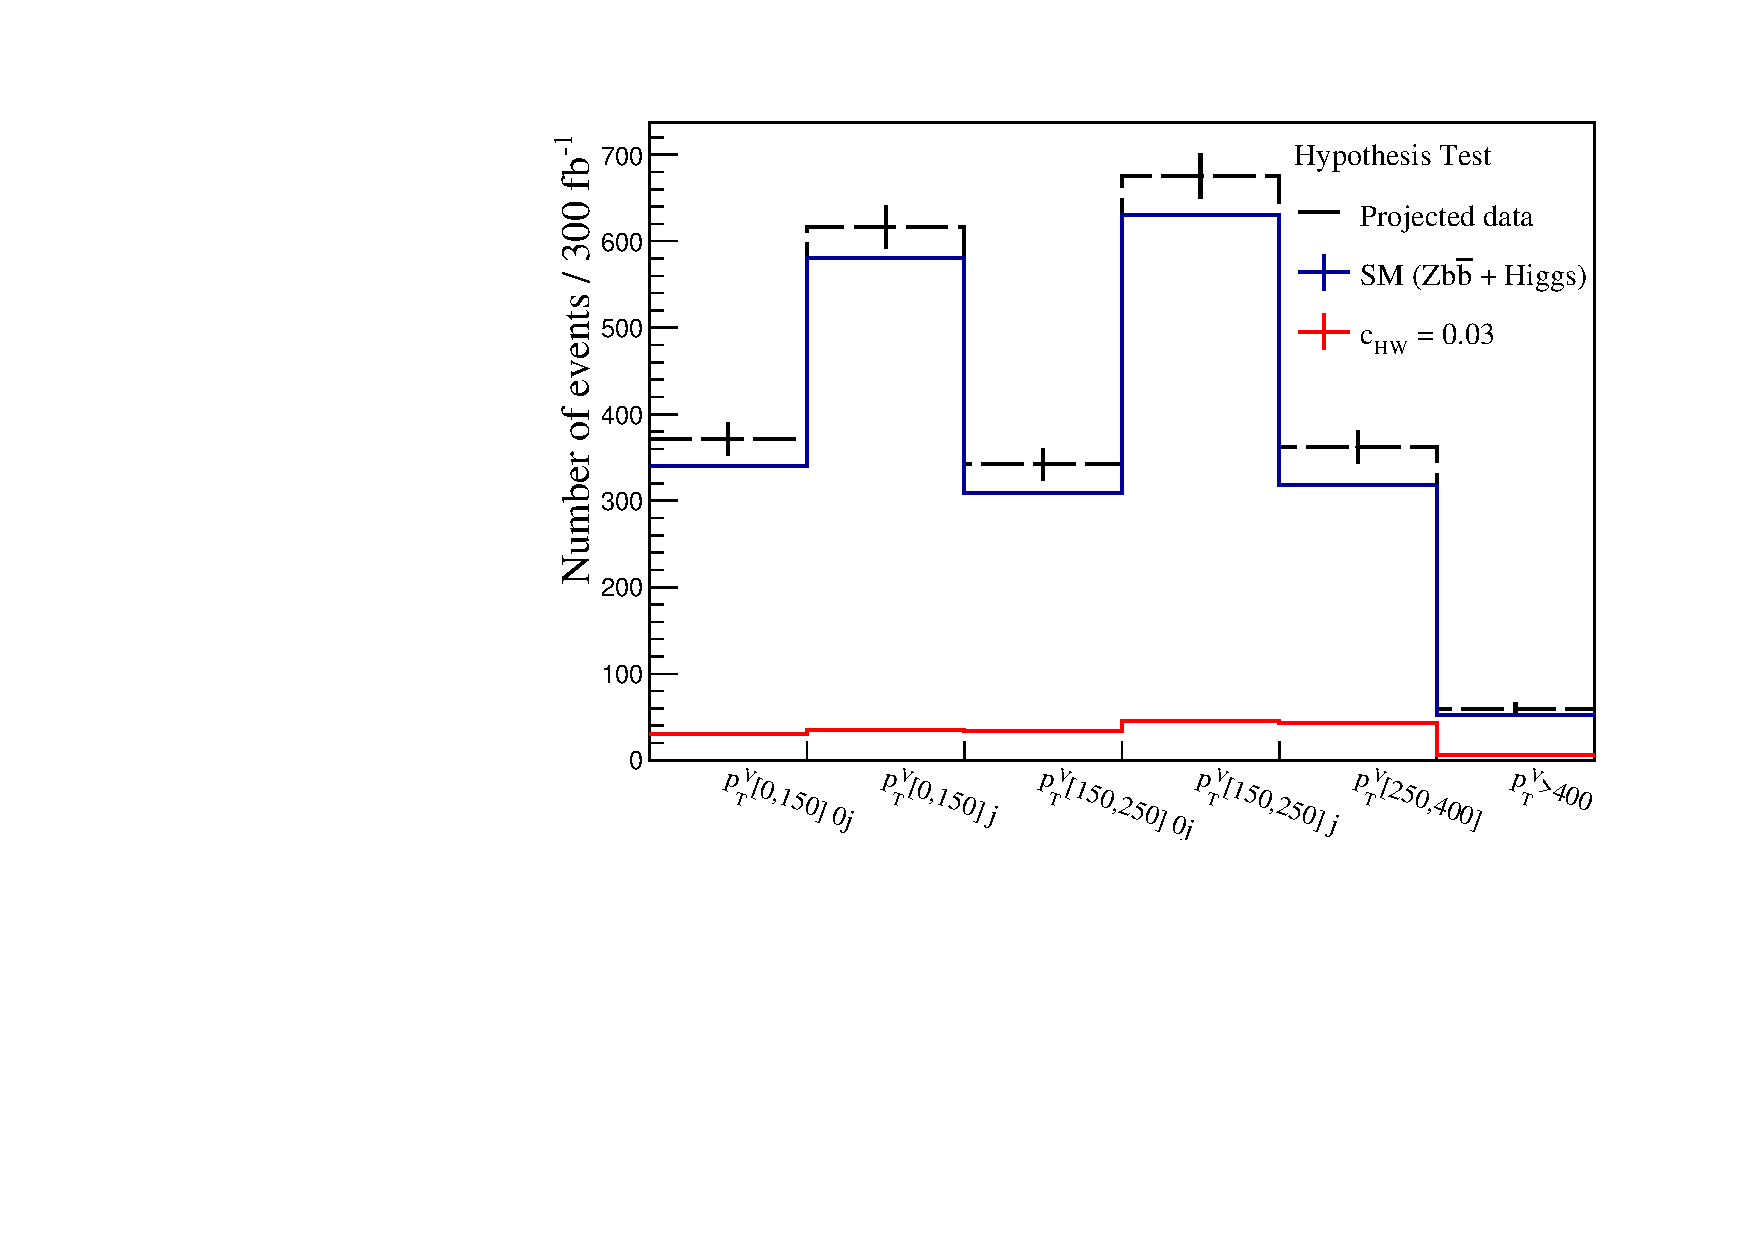
\includegraphics[width=0.45\textwidth]{plots/HypoTest_STXS.pdf}
      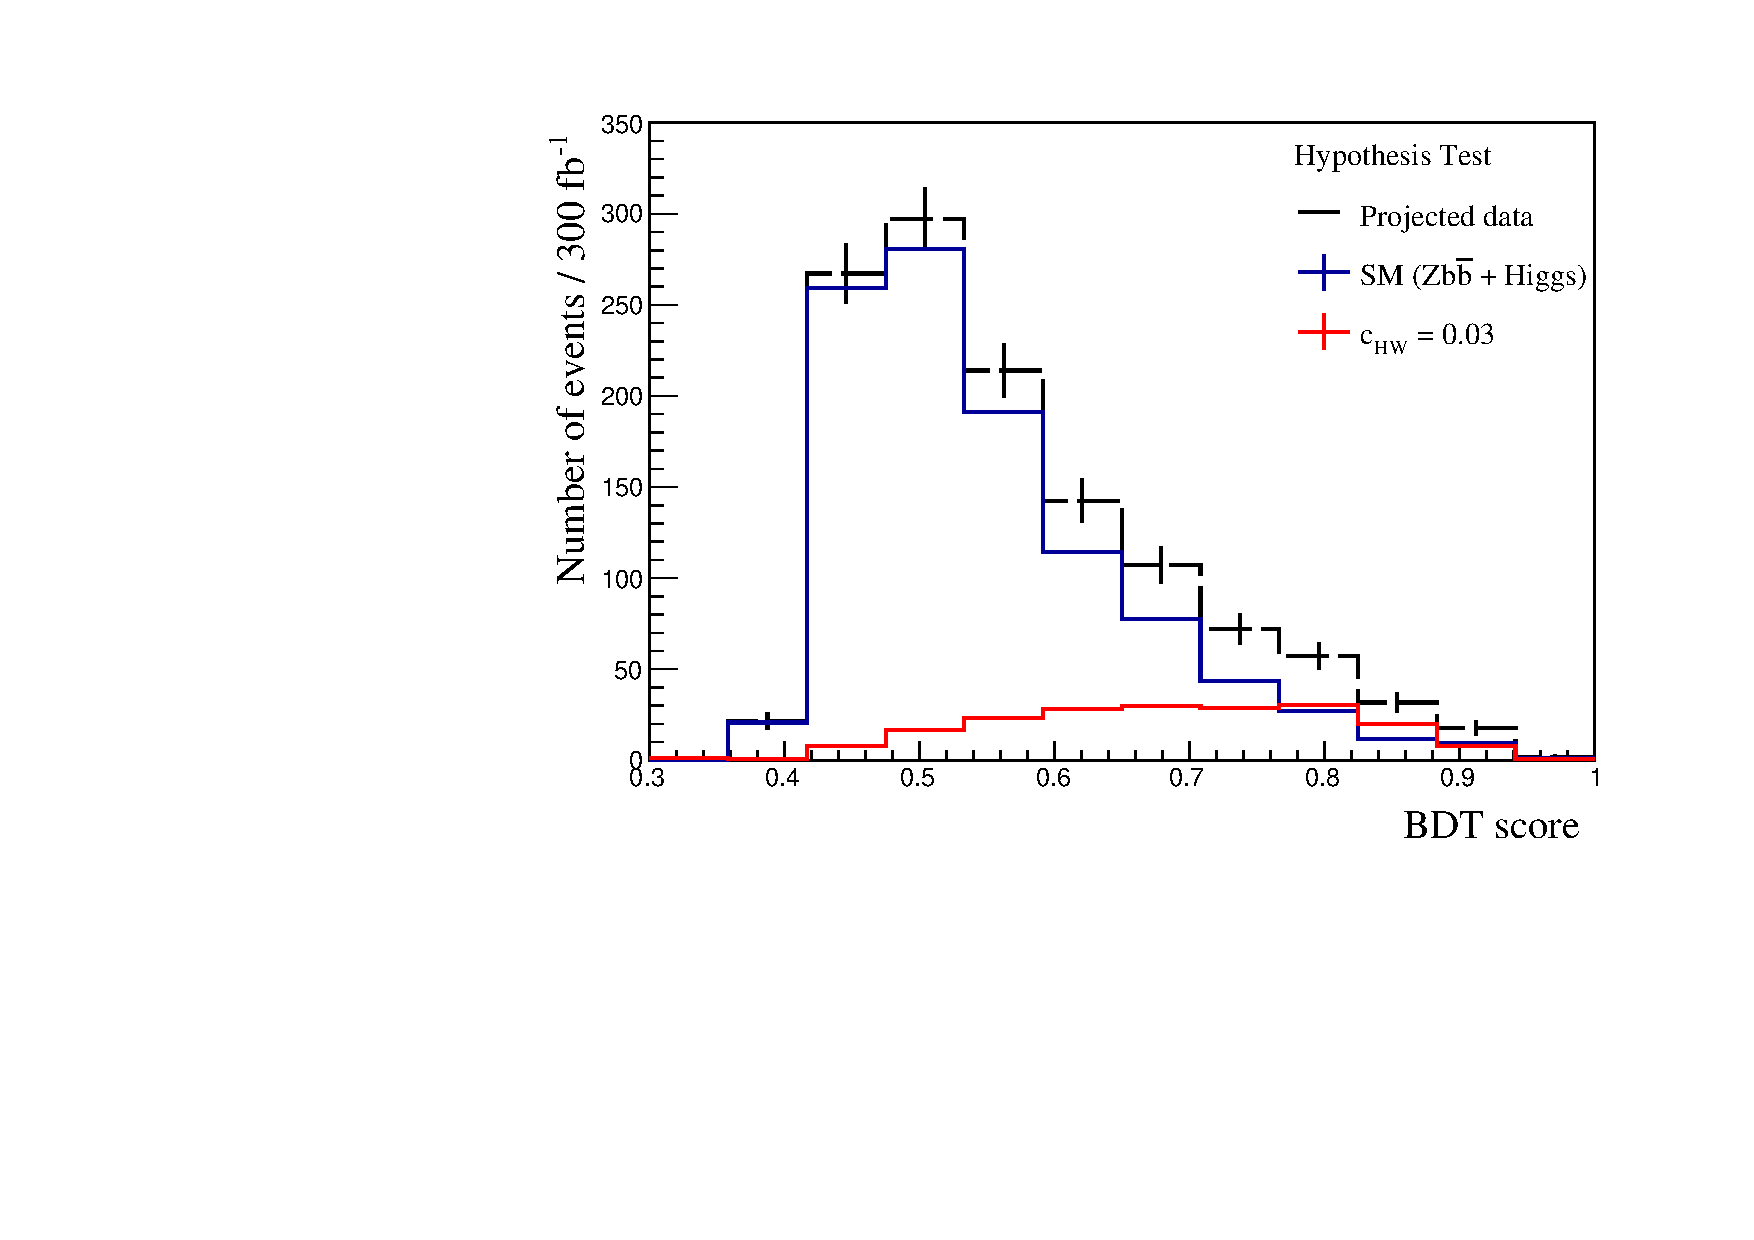
\includegraphics[width=0.45\textwidth]{plots/HypoTest_BDT.pdf}
      \caption{Predicted number of events selected for 300 fb$^{-1}$. Since the acceptance extrapolation into the STXS phase space does not change the available data statistics, it it not applied here.}
\label{fig:hypotest}
\end{figure}

Three different luminosity scenarios are investigated: the full Run-2 results, corresponding to 150 fb$^{-1}$, the integrated luminosity projected for LHC Run-3 (300 fb$^{-1}$) and the data hoped to be recorded at the High-Luminosity LHC (3000 fb$^{-1}$). To get a feeling of how realistic the scenario investigated herein is, the significance of a Higgs discovery in the STXS scenario is also investigated in addition. The expected significances for the 2-lepton channel investigated here are 1.9 for ATLAS~\ref{Aaboud:2017xsd} and 1.8 for CMS~\ref{Sirunyan:2017elk}. 
XXX compare to XX sign found here.

XXX
Table~\ref{tab:significances} summarizes the significances found  




 %c_{\sss HW} = \pm 0.03 \text{ and } \pm0.01\,,

\begin{table}[!h]
\begin{center}
{\scriptsize
\begin{tabular}{|l|c|c|c|c|c|c|c|c|c|}
\hline  
Hypothesis test		&  Full Run-2 (150 fb$^{-1}$) 	& LHC Run-3 (300 fb$^{-1}$) 	& HL-LHC  (3000 fb$^{-1}$) \\ \hline

STXS: Higgs discovery	& 		5.88		&  	7.18			&  17.41\\ \hline

STXS: $c_{\sss HW} = 0.03$ &		1.69		&	1.97			& 4.10\\
STXS: $c_{\sss HW} = -0.03$ &		0.93		&	1.12			& 2.66\\

BDT: $c_{\sss HW} = 0.03$ &		11.82		&	16.577			&  > 25\\
BDT: $c_{\sss HW} = -0.03$ &		8.2		&	11.55			& 36.21\\ \hline

BDT: $c_{\sss HW} = 0.03$ &				&				& \\
BDT: $c_{\sss HW} = -0.03$ &		0.461		&	1.55			& 7.926\\ \hline


STXS: $c_{\sss HW} = 0.01$ &				&				& \\
STXS: $c_{\sss HW} = -0.01$ &				&				& \\

BDT: $c_{\sss HW} = 0.01$ &				&				& \\
BDT: $c_{\sss HW} = -0.01$ &				&				& \\ \hline

 
\end{tabular}
}
\vskip0.5truecm
\caption{The table compares the 
}
\label{tab:significances}
\end{center}
\end{table} 
